\documentclass[11pt,letterpaper]{article}
\pdfinfoomitdate=1
\pdftrailerid{}
\pdfsuppressptexinfo=15
\usepackage[T1]{fontenc}
\usepackage[utf8]{inputenc}
\usepackage{lmodern,microtype}
\usepackage[margin=0.78in,headheight=15pt,headsep=18pt,footskip=28pt]{geometry}
\usepackage{amsmath,amssymb,graphicx,booktabs,tabularx,longtable,array}
\usepackage[table]{xcolor}
\usepackage{tikz}
\usetikzlibrary{arrows.meta,positioning,calc,fit,backgrounds}
\usepackage[most]{tcolorbox}
\usepackage{enumitem,fancyhdr,titlesec}
\usepackage[numbers,sort&compress]{natbib}
\usepackage{url}
\usepackage[font=small,labelfont=bf]{caption}
\usepackage{placeins,float}
\usepackage{hyperref}
\definecolor{ink}{HTML}{21172E}
\definecolor{violet}{HTML}{693BB7}
\definecolor{lavender}{HTML}{B39AE8}
\definecolor{night}{HTML}{100A1E}
\definecolor{mint}{HTML}{1E7153}
\definecolor{amber}{HTML}{995B13}
\definecolor{pale}{HTML}{F4F0FA}
\definecolor{muted}{HTML}{675F72}
\hypersetup{colorlinks=true,linkcolor=violet,citecolor=violet,urlcolor=violet,
 pdftitle={BLOOM Infinity: Every Successor Must Earn Its Proof},
 pdfauthor={Vincent Boucher, MONTREAL.AI},
 pdfsubject={Verified capacity, causal artifact handoffs, and conditional value},
 pdfkeywords={BLOOM, Transformational Intelligence, SUCCESSOR Omega, dependency analysis, reproducibility}}
\urlstyle{same}
\color{ink}
\setlength{\parindent}{0pt}
\setlength{\parskip}{6pt plus 1pt}
\setlength{\emergencystretch}{2em}
\setlist[itemize]{leftmargin=1.4em,itemsep=3pt,topsep=4pt}
\setlist[enumerate]{leftmargin=1.5em,itemsep=3pt,topsep=4pt}
\renewcommand{\arraystretch}{1.17}
\newcolumntype{Y}{>{\raggedright\arraybackslash}X}
\titleformat{\section}{\sffamily\Large\bfseries\color{violet}}{\thesection}{0.55em}{}
\titleformat{\subsection}{\sffamily\large\bfseries\color{ink}}{\thesubsection}{0.55em}{}
\titleformat{\paragraph}[runin]{\bfseries}{\theparagraph}{0.5em}{}[.]
\titlespacing*{\section}{0pt}{17pt}{7pt}
\titlespacing*{\subsection}{0pt}{12pt}{5pt}
\pagestyle{fancy}\fancyhf{}
\fancyhead[L]{\sffamily\small\color{muted}BLOOM $\infty$ \enspace / \enspace VERIFIED CAPACITY}
\fancyhead[R]{\sffamily\small\color{muted}MONTREAL.AI}
\fancyfoot[L]{\sffamily\footnotesize Independent research edition 1}
\fancyfoot[R]{\sffamily\footnotesize\thepage}
\renewcommand{\headrulewidth}{0.25pt}
\newtcolorbox{evidencebox}[1]{enhanced,colback=pale,colframe=violet!35,boxrule=.45pt,
 arc=2mm,left=3mm,right=3mm,top=2mm,bottom=2mm,title={#1},fonttitle=\sffamily\bfseries,
 coltitle=ink,colbacktitle=violet!8,breakable}
\newcommand{\bloom}{\textsc{BLOOM}$\infty$}
\newcommand{\pass}{\textcolor{mint}{\textbf{PASS}}}
\newcommand{\miss}{\textcolor{amber}{\textbf{FAIL}}}
\graphicspath{{figures/}}
\begin{document}
\hypersetup{pageanchor=false}
\begin{titlepage}
\begin{tikzpicture}[remember picture,overlay]
\fill[night] (current page.south west) rectangle (current page.north east);
\foreach \x/\y/\r in {1.0/1.2/.022,2.2/2.8/.015,4.6/1.1/.018,6.8/3.4/.025,8.4/1.8/.015,12.2/2.1/.028,16.9/3.1/.018,18.4/1.3/.02,1.8/8.5/.018,5.7/9.8/.022,13.8/9.5/.016,18.2/8.7/.024,16.5/15.1/.02,19.1/19.4/.018,15.2/23.0/.018,4.2/23.9/.024,1.5/20.5/.018}
 {\fill[lavender!75] ($(current page.south west)+(\x cm,\y cm)$) circle (\r cm);}
\draw[violet!60,line width=.5pt] ($(current page.south east)+(-1.5cm,9.9cm)$) circle (3.2cm);
\draw[violet!35,line width=.5pt] ($(current page.south east)+(-1.5cm,9.9cm)$) circle (4.25cm);
\draw[lavender!25,line width=.5pt] ($(current page.south east)+(-1.5cm,9.9cm)$) circle (5.3cm);
\node[draw=lavender,fill=violet!35!night,circle,minimum size=1.15cm,text=white,font=\sffamily\bfseries]
 (k) at ($(current page.south west)+(11.7cm,9.9cm)$) {$K$};
\node[draw=lavender,fill=night,circle,minimum size=1.15cm,text=white,font=\sffamily\bfseries]
 (s) at ($(current page.south west)+(16.3cm,9.9cm)$) {$S$};
\draw[-{Stealth[length=3mm]},lavender,line width=1pt] (k)--node[above,text=white,font=\sffamily\small]{verified artifact}(s);
\node[text=lavender,font=\sffamily\small] at ($(current page.south west)+(11.7cm,8.8cm)$) {CAPABILITY};
\node[text=lavender,font=\sffamily\small] at ($(current page.south west)+(16.3cm,8.8cm)$) {SUCCESSOR};
\node[text=white,font=\sffamily\small] at ($(current page.south west)+(14cm,7.85cm)$) {Fresh task. Fresh proof. Explicit authority.};
\end{tikzpicture}
\color{white}\sffamily
\vspace*{0.25in}
{\small\textls[160]{MONTREAL.AI \quad / \quad RESEARCH 2026}}\par
\vspace{0.65in}
{\fontsize{66}{70}\selectfont\bfseries BLOOM $\boldsymbol\infty$}\par
\vspace{0.32in}
{\fontsize{30}{39}\selectfont\bfseries EVERY SUCCESSOR\\MUST EARN ITS PROOF.\par}
\vspace{0.38in}
{\Large\color{lavender}Verified capacity. Conditional value.}\par
\vspace{0.25in}
\begin{minipage}{0.78\textwidth}
{\large A preregistered study of selective operator construction, causal artifact handoffs, and the measured operational cost of qualified succession.}
\end{minipage}
\vfill
{\small\textls[100]{AGI ALPHA AGENT \quad | \quad TRANSFORMATIONAL INTELLIGENCE $\infty$}}\par
{\small SUCCESSOR $\Omega$ \enspace / \enspace Local Harness integration}\par
\vspace{0.28in}
{\large Vincent Boucher \enspace $\cdot$ \enspace MONTREAL.AI}\par
{\small 23 October 2026, Montr\'eal \quad / \quad Independent research edition 1}\par
\vspace{0.15in}
{\footnotesize Research program: \emph{The seed that invents its economy}.\\This edition establishes a bounded engineering result; competitive and commercial targets remain evidence-gated.}
\end{titlepage}
\setcounter{page}{1}
\hypersetup{pageanchor=true}
\section*{Abstract}
Software teams repeatedly ask which applications a dependency change can affect and what coverage work should follow. Recomputing every answer wastes work; trusting a portable result after its conditions change can produce a confident error. We implement \bloom, a local system that constructs a graph-specific impact operator, verifies its exact domain, and passes its answers to a distinct minimum-cost coverage-planning successor. The system uses unchanged published AGI ALPHA / SUCCESSOR $\Omega$ runtime components, with inspectable native history and inactive restoration. Before confirmation, we freeze source, analysis and a balanced 48-world study; an independently executed 24-world shifted-size set and a complete deterministic replay follow. All 2,016 eligible confirmatory trials resolve exactly, all 288 input/authority refusals are correct, and all 144 conventional replacement artifacts are accepted. Removing receiver-proof checks causes 48/48 adversarial trials to accept incorrect outcomes. The performance verdict in the shared study runner is narrower: CPU point estimates improve by 2.9\% against an expert-style policy and 4.2\% against reverse indexing, but neither establishes the prespecified 10\% advantage. Artifact retention reduces receiver CPU by 22.2\% at the point estimate; its Bonferroni-adjusted percentile interval supports 19.4--24.9\%, narrowly missing the required 20\% lower bound. Fresh reproduction also misses the practical thresholds. A real public-manifest demonstration covers 1,136 nodes and 2,000 edges through seven native stages. Cash revenue is zero; complete monetary cost and demand are unmeasured. The contribution is an exact, portable and reproducible engineering system with prospective causal evidence and explicit limits, not a new reachability algorithm or proven autonomous commerce.

\begin{evidencebox}{The measured verdict}
\begin{tabularx}{\linewidth}{@{}lY@{}}
\textbf{Earned} & Exact supplied-graph outcomes; qualified artifact transport; correctly bounded restoration; reproducible local execution.\\
\textbf{Not established} & The declared 10\% competitive advantage; the declared 20\% minimum receiver gain; full-cost commercial viability.\\
\textbf{Useful today} & Inspect public dependency impact and a finite coverage plan, export the evidence, and restore its history without inheriting authority.\\
\end{tabularx}
\end{evidencebox}
\smallskip
{\small\textbf{Evidence identity.} Freeze manifest: \texttt{ecd3df27\ldots1116bcfbe}; 48 confirmatory worlds; 24 fresh reproduction worlds; 2,544 deterministic replay records. Full identities and commands appear in Section~\ref{sec:reproduction}.}
\clearpage
\section{The capacity that survives a completed task}
An accepted output can be useful in two ways. It may answer the present question, and it may supply a capability that changes the work required by a later question. The second value is conditional. Construction has a cost. Verification has a cost. A changed graph, a revised policy, or withdrawn permission can invalidate the receiving use. A successor must therefore earn its own proof.

This research starts with a practical, nonpersonal need in the project's public software: determine which application roots depend on a changed package, then produce an inspectable coverage plan for those roots. The first task is graph reachability. The second is finite weighted coverage. The successor reads an actual predecessor-produced impact artifact; it does not receive a fictional mission label or a presumed financial return.

TRANSFORMATIONAL INTELLIGENCE supplies the motivating question: can changing the problem-solving setup make a purpose easier to achieve without weakening that purpose? The transformation here is bounded and concrete. Repeated traversal can be replaced by a graph-specialized data program with independently checked applicability. Its usefulness depends on the workload and on the cost of keeping its proof current. The foundations distinguish this structural question from a claim of novel unrestricted planning or universal superiority~\cite{boucher2026ti,boucher2026execute,boucher2026economy}.

The strongest ordinary method remains eligible. BLOOM may use direct traversal, memoization, component propagation, reverse indexing or finite Warshall closure. The conventional references receive the same choices, information and qualification criteria. Building something new is a conditional option, never a requirement for an impressive-looking trace. In the real-manifest demonstration, the expert-style policy selects conventional reverse indexing.

\subsection{Contribution statement}
This edition contributes four connected artifacts. First, it implements a source-bound portable impact operator with exact certificates and a separately checked coverage successor. Second, it contributes a timestamped, preregistered comparison that distinguishes competitive advantage from the causal benefit of retaining an artifact. Third, it exercises the published Alpha dispatcher, real native history, backup and restoration in a bounded local journey. Fourth, it delivers complete source, raw observations, independent checks, a public-manifest example and an inspectable evidence browser.

The verification propositions collect sufficient conditions for the implemented certificates. They are engineering arguments built from established graph techniques, not claims that SCC decomposition, dynamic programming, caching, algorithm selection or test coverage were invented here. Earlier project editions develop mission-relative capability inheritance and construction of a next capability~\cite{montrealai2026writer4,montrealai2026writer5}. This edition starts its own problem, generator and comparative design, and adds controlled retention, replacement, corruption and resource interventions. No learned model constructs a new algorithm during the confirmatory run. The implemented construction specializes a maintained operator grammar to a particular graph; every resulting program remains finite and inspectable.

\subsection{Three distinct meanings of success}
\textbf{Engineering success} means exact results within the stated contract, readable failures, reproducible commands, preserved evidence and honest authority. \textbf{Scientific advantage} means passing the declared comparative thresholds against strong allowed alternatives. \textbf{Economic success} would additionally require supported demand and complete attributable costs. The first can be delivered while the latter two remain unproven. The paper keeps all three verdicts visible.

\paragraph{Research question} Under changing workload and resource constraints, does constructing and carrying a verified graph-specific operator improve complete operational cost over equally equipped conventional methods, and does its artifact causally reduce the work of a distinct successor? The answer is tested with declared practical thresholds; useful exactness alone cannot answer the comparative question.

\section{Problem, operators, and qualified succession}
\label{sec:bloom-formal}

The operational principle of \textsc{BLOOM}$\infty$ is that every successor must earn its proof. In this study, the predecessor supplies a reusable dependency-impact operator; the successor uses its answers to construct a finite coverage plan. These are distinct tasks connected by consumed data. Neither a lineage label nor successful execution of the predecessor establishes the successor's validity.

Let $G=(V,E)$ be a finite directed graph, with $u\to v$ meaning that $v$ depends on $u$. Let $A=(a_0,\ldots,a_{k-1})$ be the ordered application list. For a changed-node set $S\subseteq V$, the impact target is
\begin{equation}
 I_G(S)=\{a\in A:\exists s\in S,\ s\leadsto_G a\},
\end{equation}
where reachability includes paths of length zero. A node therefore affects itself when it is an application. The ordering of $A$ defines bit positions and is part of the artifact binding. We write $R(v)$ for the bitmask encoding $I_G(\{v\})$; a multi-source answer is the bitwise union of its source masks.

The successor receives tests $\mathcal{T}$, coverage sets $C_t\subseteq A$, and strictly positive integer weights $c_t$. For an impact set $I$, it computes
\begin{equation}
 J^*(I)\in\mathop{\arg\min}_{J\subseteq\mathcal{T}}
 \left\{\sum_{t\in J}c_t:I\subseteq\bigcup_{t\in J}C_t\right\}.
\end{equation}
Equal-cost solutions use the lexicographically smallest tuple of sorted test identifiers. Empty impact produces the empty feasible plan; uncovered requirements produce an explicit infeasible result. The implementation bounds cases to ten applications and twelve tests; the synthetic instances use six applications and ten tests, permitting exact finite optimization. Weights are declared synthetic durations, not measured test runtimes or money. Coverage of these requirements does not establish preservation of every fault detectable by the original test suite~\cite{rothermel1997safe,harrold1993reduction}.

The schema \texttt{bloom-impact-operator/v1} stores a strategy, ordered applications, rows, certificate, and world, policy, environment and source digests. It declares \texttt{authority: none}. A compiled row index is a data-specialized operator executed by a fixed interpreter. Its graph-specific contents are constructed during the run; the underlying algorithms and interpreter are maintained software. This is finite specialization, not discovery of a new graph algorithm or unconstrained program synthesis.

\subsection{Certificates establish exactness, not merely closure}
\label{sec:bloom-certificates}

There are two complete-index certificates. Both are checked against the supplied graph rather than a producer-provided edge summary. Range, dimension, partition and integer-type checks precede the semantic checks. In particular, a content digest alone supplies no reachability proof.

\paragraph{Proposition 1: component recurrence}
Suppose a certificate partitions $V$ into nonempty sets $\mathcal{P}$; every set induces a strongly connected subgraph; and every edge between distinct sets advances in a supplied topological order. For $C\in\mathcal{P}$, let $L_C$ encode the applications inside $C$. Suppose the verifier establishes
\begin{equation}
 B_C=L_C\mathbin{\lor}\bigvee_{(C,D)\in E_{\mathcal P}}B_D
 \quad\text{and}\quad R(v)=B_C\quad(v\in C),
 \label{eq:bloom-scc-recurrence}
\end{equation}
where $E_{\mathcal P}$ is reconstructed from $E$. Then every row is exactly the reachable-application mask of its node.

\paragraph{Proof}
Forward and reverse traversal within a proposed component, from one representative, establish that every member reaches every other member. The checked topological order makes the quotient graph acyclic. A path from any member of $C$ to an application either stays in $C$ or first exits along an edge to a successor component. Conversely, strong connectivity lets every member reach the tail of each such exit. Thus the reachable applications satisfy precisely Equation~\ref{eq:bloom-scc-recurrence}. Reverse topological induction gives its unique solution, beginning with sinks, whose masks contain only their local applications. Equality of every node row with its component mask completes the argument. This verifies both absence of spurious applications and inclusion of every reachable application.\hfill$\square$

The implementation constructs components by two graph traversals and propagates application masks over the condensation. The independent verifier checks the partition, induced strong connectivity, topological edges and recurrence afresh. For the bounded application count, structural verification is linear in graph and certificate size; larger masks add their explicit bit-operation cost. Strong-component computation and transitive closure are established techniques~\cite{tarjan1972dfs,warshall1962boolean}.

\paragraph{Proposition 2: reverse-path witnesses}
Alternatively, suppose each application owns its own bit. For every claimed bit $a\in R(v)$ with $v\ne a$, the certificate supplies an actual edge $v\to p_a(v)$, the same claimed bit at $p_a(v)$, and nonnegative integer ranks satisfying $r_a(v)>r_a(p_a(v))$. The application root points to itself with rank zero. Unclaimed bits have absent witnesses. Finally, every graph edge $u\to v$ satisfies $R(v)\subseteq R(u)$. Then the rows encode exactly all reachable applications.

\paragraph{Proof}
For a claimed bit, following its witness strictly decreases a nonnegative rank. It cannot continue indefinitely or cycle; a nonroot cannot terminate at rank zero because its required successor would have a smaller nonnegative rank. The chain therefore reaches the corresponding application through actual edges. There are no false positives. For the opposite direction, a path $v=v_0\to\cdots\to v_\ell=a$ starts from the application's required ownership bit. Repeated edge closure propagates that bit backward to every $v_i$, including $v$. There are no false negatives.\hfill$\square$

Reverse traversal from each application constructs these witnesses alongside the index. The verifier performs $O(k|V|+|E|)$ structural checks, with arithmetic cost determined by encoded integers and masks. Ordinary edge closure without the descending witnesses would accept an all-ones overapproximation; witnesses supply the missing inclusion in the true reachability relation. Memoized operators instead advertise partial rows, each replayed against independent BFS. Every memoized and direct output also receives fresh BFS checking, including cached outputs.

\subsection{Construction and conventional alternatives}

The candidate and expert selection policies can choose direct traversal, memoization, component propagation, reverse-per-application indexing and bitset Warshall closure. The second reference deliberately follows a fixed reverse-index strategy, with memoization then direct traversal as its legal fallbacks. It has the same information and wrapper, while the full-palette expert provides the primary equally equipped competitor. All receive the complete query batch, current graph, applications, test catalogue, available constructors and payload cap. A shared wrapper charges construction attempts, checks actual canonical serialized bytes, and records fallback to an available memoized or direct operator. The cap is not a claim about resident memory.

The candidate uses frozen graph-work estimates and requires at least 20\% estimated headroom before preferring component or Warshall specialization over its available conventional alternatives. This threshold is a policy assumption, not an observed CPU saving. The estimates approximate graph work; they do not price all certificate, integration, maintenance or failure-risk costs. The policy therefore approximates the binding computational constraint rather than solving a complete expected-value optimization. The measured end-to-end test is deliberately able to reject its usefulness. An independently written expert-style policy uses its own transparent workload estimates over the same palette. A conventional reverse-index policy is the second reference. The constructors and qualification boundary are shared deliberately: the comparison tests the policies within this implementation envelope, not differently optimized reimplementations of the same primitives. No claim is made that the reference is the globally fastest existing package. Practical reachability work already demonstrates the importance of initialization, update and query tradeoffs~\cite{hanauer2020dynamic}.

\section{Prospective comparison and artifact interventions}
\label{sec:bloom-methods}

Competitive advantage and artifact dependence are different estimands. For world $w$, let $T_{B,w}$ and $T_{C,w}$ denote complete measured operational CPU for candidate and conventional policies. The competitive ratio is
\begin{equation}
 \rho_C=\exp\left(\frac{1}{W}\sum_{w=1}^{W}
 \log\frac{T_{B,w}}{T_{C,w}}\right).
\end{equation}
Both policies have the same artifact and construction opportunities. Separately, let $S_w(K)$ be receiver CPU with the qualified predecessor artifact retained, and $S_w(\varnothing)$ receiver CPU when it is withheld and reconstruction remains allowed. Their paired ratio tests saved receiver work. Total predecessor-plus-receiver CPU is also reported. An artifact-deprived receiver is an intervention arm, not the principal competitive baseline. This explicit separation follows the logic of defining causal treatments before inspecting outcomes~\cite{rubin2008design}.

The protocol reserves twelve development worlds, at most two versioned development cycles, 48 confirmatory worlds and 24 fresh reproduction worlds. Confirmation crosses four topologies, four node counts and three query-batch sizes. Reproduction crosses the same topologies and query counts with two shifted sizes. The graph world is the independent unit; repeated queries and derived stages are not additional independent observations. The generator and seed ranges are known to the authors. Confirmation uses seeds 20001--20048; reproduction uses 30001--30024. The topologies are sparse DAG, layered DAG, hub graph and cyclic modules; node counts are 48, 72, 96 and 128 in confirmation and 64 and 160 in reproduction, with query batches of 8, 32 and 96. This is untouched execution under a disclosed generator, not a concealed external benchmark. Protocol, source and analysis were frozen and durably persisted before confirmation, preserving the distinction between declared tests and later explanation~\cite{nosek2018preregistration}.

Stable and withheld arms use three complete timed replicates with reset method-local state and randomized execution order. The direct-walk no-construction arm and the proof-disabled corruption diagnostic each use one execution per world. Other declared interventions use one execution: conventional replacement, graph change, rehashed semantic corruption, policy change, authority revocation, scarce storage, constructor outage, withholding combined with outage, malformed input, infeasible coverage, and incomplete observed dependencies. A constructor outage does not invalidate a previously constructed data operator; it restricts new construction. The policy-change case removes a test from the eligible catalogue. Corruption modifies a supplied mask and recomputes its content hash, testing semantics rather than accidental checksum failure. Interventions occur before receiver execution.

Five gates separate reproducibility, quality, competition, succession and economics. Deterministic records must replay exactly, excluding timing and host-dependent metadata. Every eligible complete-graph task must resolve correctly, including explicit infeasibility; authority and malformed-input refusals are evaluated separately. The primary competitive endpoint uses only stable authorized worlds and the median of three complete CPU observations. It includes validation, policy choice, attempted construction, operational qualification, transport, revalidation and successor checking. The native seven-stage orchestration is measured separately in the practical demonstration, not inserted into every scientific kernel trial. Thus these primary times cover the full declared runner operation, not the full product stack. A separately measured research audit uses independent BFS and exhaustive subset enumeration; it is excluded symmetrically from method latency and included in research cost.

Competitive success requires a simultaneous upper ratio bound below $0.90$ against both conventional references without loss of correctness or completion. Artifact benefit requires a receiver ratio bound below $0.80$ at equal quality. The three contrasts form one family: 10,000 fixed-seed world-bootstrap replicates~\cite{efron1979bootstrap} produce 98.333333\% two-sided percentile intervals, providing nominal Bonferroni family coverage of 95\%. Bootstrap coverage is approximate. A subgroup or inner-kernel improvement cannot replace the primary verdict. Scientific execution is capped at 1,200 CPU seconds and 256 MiB of new evidence; interrupted campaigns retain incomplete denominators and failed attempts.

\subsection{Boundaries of independence and proof}

The checker was authored separately within the same research session. Its BFS, finite subset enumeration, and certificate checks do not import candidate kernels. This reduces shared implementation error but is neither organizational independence nor a blinded external evaluation. Reproduction in another process establishes reproducibility under recorded conditions, not universal portability.

World, policy, proof and authority remain separate predicates. The receiver serializes and reopens the artifact, checks current graph/application, policy and source/environment bindings, and rechecks semantics. Restored history has no active proof or grant. Revoked receiver authority requires refusal even after legitimate predecessor production. Missing edges illustrate the observability boundary: exactness over an incomplete supplied graph can still omit real impact. The intervention reports that limitation instead of treating a valid hash as evidence of graph completeness.

The project stages are a trace through these operations: Identify binds the need; Out-Learn reads declared structure; Out-Think compares eligible operators; Out-Design constructs only when justified; Out-Strategise binds constraints; Out-Execute qualifies and computes; Out-Evolve evaluates the distinct coverage successor and retains or terminates its history. These labels do not enlarge the native runtime's authorization or make a changed plan inherit an earlier proof.

\section{Relation to established work}
\label{sec:bloom-related}

Instance-conditioned operator choice is algorithm selection~\cite{rice1976selection}; parameter and procedure tuning have extensive configuration literature~\cite{hutter2011smac}. Reusable program libraries and construction of later solutions from earlier abstractions are also established~\cite{ellis2021dreamcoder}. Here, the contribution sought is controlled evidence about when a qualified, portable operator pays for its complete measured operational cost and enables a successor under explicit constraints. The familiar machinery is identified rather than renamed as a discovery.

Coverage reduction has a longstanding test-to-requirement formulation~\cite{harrold1993reduction}. Weighted greedy set cover provides an important scalable conventional alternative~\cite{chvatal1979cover}; this experiment uses exact optimization only because its catalogue is deliberately small and grants the same optimizer to every policy. Safe regression selection has stronger assumptions and goals than coverage preservation~\cite{rothermel1997safe}. Consequently, no synthetic planning weight is reported as measured testing saved or preserved fault detection. Finally, portable experiment packaging and provenance precede this work~\cite{chirigati2013reprozip}. Exportability preserves inspectable evidence; semantic applicability and authority must still be established at the receiving boundary.

\subsection{What is new, and what remains established engineering}
Programming by examples can synthesize transformations within a specified grammar~\cite{gulwani2011strings}; DreamCoder extends this with learned reusable abstractions~\cite{ellis2021dreamcoder}. BLOOM's confirmatory operator grammar and construction algorithms are fixed in advance. Its new per-world object is graph-specific data plus a certificate. It does not reproduce those systems' learned program discovery, and calling this finite construction ``invention'' does not establish equivalent capability.

Workflow planning already reasons about ordered task decomposition and applicability~\cite{nau2003shop2}. Reuse of qualified components has deep engineering roots~\cite{mcilroy1968components}; content-addressed deployment and provenance support inspectable portability~\cite{dolstra2004nix,chirigati2013reprozip}. This edition's additional evidence is the explicit, prospective separation of a fair selection comparison from artifact-retention, replacement and proof-ablation interventions, connected to the project's actual native lifecycle. Its contribution is that integrated experiment and usable bounded implementation, not ownership of the underlying planning or reuse idea.

Adaptive experimentation can invalidate ordinary holdout interpretation when the same evaluation answers guide repeated selection~\cite{dwork2015holdout}. Here, twelve development worlds support two visible development cycles; no confirmatory outcome is used to revise the policy. The fresh-size set remains separately reported after the original failure. The resulting procedure is a simple frozen-split design, not a new reusable-holdout method. The paper's negative comparative result is part of the contribution.

\FloatBarrier
\section{Results: exact outcomes, unmet advantage thresholds}
\label{sec:results}
The confirmatory campaign contains 48 independent graph worlds and 2,544 trial executions. The fresh reproduction contains 24 worlds and 1,272 trials. A further 2,544 executions replay the original confirmation; they add computational cost, not independent worlds. All planned trial keys are present. Raw records, case files, operator artifacts, replacement receipts and the frozen analysis are retained, including the diagnostic failures.

\subsection{The decision tree resolves without a superiority claim}
Table~\ref{tab:gates} gives the prespecified decision tree and its final disposition. Failure of a later gate does not erase an earlier engineering result. It prevents the stronger associated claim. The original analysis correctly leaves G1 pending until the independent replay is available; a separate content-hashed review receipt closes it. The original analysis file is not rewritten to manufacture contemporaneous certainty.

\begin{table}[htbp]
\centering\small
\begin{tabularx}{\textwidth}{@{}p{.36in}Yp{1.10in}Y@{}}
\toprule
Gate & Pass condition & Verdict & Consequence \\
\midrule
G1 & Exact deterministic replay under frozen identities & \pass & All 2,544 records, 48 cases and 480 operators match. \\
G2 & Every eligible resolution exact; expected refusals and artifact boundaries correct & \pass & Retain the bounded supplied-graph claim. \\
G3 & Upper CPU ratio bound $<0.90$ against both conventional references & \miss & No demonstrated 10\% competitive advantage. \\
G4 & Upper retained/withheld receiver ratio bound $<0.80$, at equal quality & \miss & Artifact effect is measured; required minimum gain is not established. \\
G5 & Supported demand and complete comparative costs & \textcolor{amber}{\textbf{INCOMPLETE}} & No commercial-viability or self-financing claim. \\
\bottomrule
\end{tabularx}
\caption{Prespecified gates, final evidence and failure dispositions. G1 is closed by the later independent reproduction receipt. G3 and G4 retain their failed verdicts after reproduction.}
\label{tab:gates}
\end{table}

Every eligible complete-graph trial resolves exactly: 2,016/2,016 in confirmation and 1,008/1,008 in fresh reproduction. These include correct infeasibility, not just successful plans. All 288 and 144 respective malformed-input or authority refusals are correct. All 1,008 and 504 required stale-or-withheld artifact rejections occur, and every conventional replacement is accepted: 144/144 and 72/72. These are execution counts within clustered worlds. Descriptive 95\% Wilson intervals for the proportion of worlds with all eligible outcomes correct are $[0.926,1]$ over 48 worlds and $[0.862,1]$ over 24. They do not prove a zero production failure rate.

\subsection{The practical performance hypotheses fail}
Table~\ref{tab:effects} and Figure~\ref{fig:effects} report all three declared contrasts. The intervals use the same multiplicity adjustment specified before confirmation. The candidate's 2.86\% and 4.21\% point improvements are smaller than the required 10\%. The interval against the expert policy also includes no improvement. The interval against reverse indexing excludes parity on this run, but excludes the required 10\% saving as well. A statistically distinguishable small difference is not the declared practical success. A descriptive hindsight oracle, selecting the faster conventional median separately in each world, averages 4.0731\,ms; BLOOM/oracle geometric ratio is 0.9983. On fresh reproduction, the oracle averages 4.4977\,ms and the ratio is 1.0378. This predeclared descriptive lower bound is computed in supplementary reporting from frozen arrays, carries no new hypothesis test, and is not an executable policy: its selection information and cost are unavailable prospectively.

\begin{table}[htbp]
\centering\small
\begin{tabular}{@{}llrrr@{}}
\toprule
Set & CPU ratio & Estimate & Adjusted interval & Required upper \\
\midrule
Confirmation & BLOOM / expert & 0.9714 & [0.9375, 1.0051] & $<0.90$ \\
48 worlds & BLOOM / reverse & 0.9579 & [0.9156, 0.9979] & $<0.90$ \\
 & Retained / withheld receiver & 0.7780 & [0.7508, 0.8059] & $<0.80$ \\
\addlinespace
Reproduction & BLOOM / expert & 1.0079 & [0.9653, 1.0725] & $<0.90$ \\
24 fresh worlds & BLOOM / reverse & 0.9608 & [0.8651, 1.0483] & $<0.90$ \\
 & Retained / withheld receiver & 0.8051 & [0.7639, 0.8552] & $<0.80$ \\
\bottomrule
\end{tabular}
\caption{All prespecified primary contrasts. Ratios below one favor BLOOM or retention. Each interval has nominal 98.333333\% coverage; the three-contrast family has nominal 95\% Bonferroni coverage. Percentile-bootstrap coverage is approximate. No row passes its practical threshold.}
\label{tab:effects}
\end{table}

\begin{figure}[H]
\centering\includegraphics[width=0.92\textwidth]{fig01_effects.pdf}
\caption{Effect estimates against the actual decision thresholds. Confirmation and fresh reproduction remain separate; pooling them after a failure would change the declared test. Source: frozen analyses, with the later independent G1 receipt shown only as provenance.}
\label{fig:effects}
\end{figure}

The arithmetic mean of the per-world median operational CPU is 4.0863\,ms for BLOOM, 4.1929\,ms for the expert policy, and 4.2568\,ms for reverse indexing in confirmation. These means describe absolute cost; the geometric paired ratios answer the primary relative question. On fresh shifted-size worlds the corresponding means are 4.6993, 4.6306 and 4.9114\,ms. The expert policy is then faster than BLOOM at the point estimate. Small Python workloads, interpreter overhead and host scheduling limit the portability of these timing magnitudes.

Both BLOOM and the expert choose SCC propagation on all 48 stable confirmatory worlds and all 24 reproduction worlds. There is no evidence here that the candidate identifies a superior standard-case operator. Its small timing differences arise within the same shared construction and verification pipeline, with different policy work and execution noise. The reverse baseline uses reverse indexing throughout. Figure~\ref{fig:choices} shows where constraints actually change behavior: payload scarcity and lack of an available constructor require ordinary fallbacks. The experiment did not create an artificially weak comparator to produce an invention win.

\begin{figure}[H]
\centering\includegraphics[width=0.92\textwidth]{fig02_cpu_phases.pdf}
\caption{Complete operational cost by phase. Each world contributes its observed median-total-CPU replicate; all phase values come from that same replicate. Means therefore add exactly to the reported total, including the measured residual. Withholding adds receiver reconstruction while predecessor creation remains charged. This is an absolute-cost description, not an additional hypothesis test.}
\label{fig:phases}
\end{figure}

\subsection{A useful artifact is not an irreplaceable artifact}
The retained/withheld intervention estimates a controlled benefit of carrying a verified operator into the receiver. Retention improves receiver CPU by 22.20\% at the confirmatory point estimate. Its adjusted saving interval is 19.41--24.92\%; the required lower bound was 20\%. The point estimate crosses the goal while the interval does not. G4 therefore fails. Fresh reproduction yields a 19.49\% point saving with a 14.48--23.61\% interval, also below the declared criterion.

The dependency itself is concrete: the coverage successor consumes the predecessor's impact artifact and its digest. Holding the graph and query fixed while removing that artifact forces reconstructive work. But successful conventional replacement in every declared replacement trial shows that the producer's identity is not necessary. The useful object is a qualified capability with the correct contents and bindings. We claim neither exclusive transfer nor a monopoly on successor creation.

These interventions are prospective controlled executions under a synthetic generator. They provide stronger evidence than retrospectively deleting a cost column from one successful trace. They still do not establish market demand, dependence in a deployed organization, or necessity when all alternative information and construction are allowed. Replacement construction is measured separately, once per actual creation, and attributed to each relevant counterfactual arm without being added repeatedly to the cash or research ledger.

\FloatBarrier
\section{Causal diagnosis and robustness}
\label{sec:causal}
The study separates three mechanisms that can easily be confused: selecting an operator, constructing its graph-specific data, and qualifying its use at a receiving boundary. The stable selection comparison offers no novel-selector advantage because the strongest policies choose the same operator. The no-construction arm answers a narrower question: what happens if the same workload always uses direct traversal? All 48 confirmatory direct arms remain exact, with mean total CPU 4.8393\,ms. This descriptive contrast suggests that specialization can save work in this finite setting. It is not the primary fair-competition test, and its single execution per world does not replace the three-replicate endpoint.

Verification has a distinct causal role. The rehashed-corruption treatment alters a real application mask and recomputes the content digest. BLOOM rejects and rebuilds all 48/48 confirmatory corrupted artifacts; all three policies do so in 144/144 verified corruption trials. In the deliberately unsafe diagnostic, disabling only receiver proof leads to 48/48 false acceptances and incorrect outcomes; fresh reproduction repeats this on 24/24 worlds. Checksums, lineage, and successful predecessor execution do not substitute for semantic revalidation. This diagnostic is not an offered operating mode.



\subsection{When exactness is insufficient}
Every method can be exact relative to a supplied dependency graph and still miss actual impact if that graph omits a real dependency. The deliberate missing-edge challenge removes incoming edges to a target application after constructing a complete hidden world, and forces the first query to node zero. The frozen protocol prose says ``removes an edge'', whereas the frozen implementation removes all incoming edges to that application. This wording mismatch is a disclosed deviation, not a random single-edge failure model; the challenge remains outside G2 and the primary timing tests. All methods omit true affected applications on 1,657 of 2,176 query instances in confirmation and 897 of 1,088 in reproduction. All 48 and 24 respective worlds exhibit omissions. These counts describe a designed stress condition, with correlated queries inside worlds; they are not prevalence estimates for public package manifests.

This is the most consequential failure mode for deployment. Better graph algorithms cannot infer undeclared runtime dependencies from a checksum. The public example is therefore an inventory of declared package relationships. It is not a certificate that an application will pass its real tests after a dependency update. Acquiring and validating representative runtime or build dependencies is a separate measurement problem.

\subsection{Changed constraints produce bounded behavior}
A graph change or policy revision invalidates the transported binding and causes fresh qualification. The policy intervention removes an actually eligible test, so the successor's feasible set changes. Authority withdrawal after legitimate predecessor production refuses the receiving execution. A 2\,KiB payload ceiling exercises failed construction and a charged conventional fallback. Constructor unavailability leaves already-constructed data usable; combining outage with withholding forces an available traversal-based replacement. Malformed inputs are rejected and uncovered requirements terminate as infeasible. None of these conditions licenses an indefinite repair loop.

\begin{figure}[H]
\centering\includegraphics[width=0.92\textwidth]{fig03_robustness.pdf}
\caption{Robustness includes correct refusals and visible failures. An infeasible world contains at least one correctly infeasible query and may also contain feasible ones. Missing edges are evaluated against the complete hidden graph, outside the supplied-graph guarantee. The proof-disabled corruption arm is deliberately unsafe. Source: complete confirmatory records, not selected successful traces.}
\label{fig:robustness}
\end{figure}

\begin{figure}[H]
\centering\includegraphics[width=0.92\textwidth]{fig04_operator_choices.pdf}
\caption{Actual strategy choices. The same strong SCC choice dominates stable conditions for BLOOM and expert. Constraints make conventional fallback visible. All methods have the same allowed palette and payload checks; a rejected build is charged and recorded. Counts are worlds, not claims of independent stages.}
\label{fig:choices}
\end{figure}

\subsection{Failure severity and what was not measured}
The implemented boundary distinguishes an incorrect accepted answer, an unnecessary refusal, a correct refusal, correct infeasibility, and incomplete observed world data. In the authorized complete-graph arms there are no incorrect accepted outcomes or unexpected refusals. Semantic corruption without receiver proof is a severe false acceptance. Incomplete-world omission is a severe external-validity limitation even when the supplied-graph proof passes. Neither category is hidden inside an average quality score.

Memory evidence is also limited. Canonical artifact bytes and the process high-water RSS are recorded; a serialized payload cap does not measure per-method resident memory. CPU and monotonic wall time are measured separately. Counter events such as traversed edges, row checks and subset scores are not interchangeable resources and are never summed into a fictional price or detector acquisition count.

\FloatBarrier
\section{Economics: conditional value, incomplete full cost}
\label{sec:economics}
The research records no cash revenue, firm offer, independently supported demand, or external customer acceptance. No financial transaction or new paid infrastructure purchase was performed. Those observations do not make authoring, execution or maintenance free. Human effort, model/service authoring, inherited hardware and integration maintenance have unknown attributable fees. G5 is therefore incomplete.

The scientific campaign ledger sums each completed campaign receipt once: 47.8877 CPU seconds across preserved development, confirmation, fresh reproduction and exact replay. External correctness audits account for 5.3831 seconds within that total, not in addition to it. Five distinct measured native integration runs separately total 6.1983 CPU seconds, including the 1.1277-second public demonstration. Three initial development calls add 0.1802 seconds. The resulting documented-compute subtotal is 54.2661 seconds. The protocol prose said native overhead was included in campaign cost; the campaign receipts actually exclude it. The final ledger explicitly includes that separate subtotal rather than rewriting the original receipts. Figure generation, document production, unmetered authoring and other integration preparation are outside that measured campaign total and remain explicit unpriced work. The ledger does not present this documented subtotal as the complete cost of producing the research.

\begin{table}[htbp]
\centering\small
\begin{tabularx}{\textwidth}{@{}p{1.8in}Yp{1.25in}@{}}
\toprule
Quantity & Evidence and interpretation & Classification \\
\midrule
Revenue / firm offers & Zero recorded; no transaction or offer validation & Observed absence \\
CPU / wall time & Per phase, trial and completed campaign; audit subsets reconcile & Measured resources \\
Detector acquisitions & Zero; no physical detector or exposure experiment & Observed count \\
Coverage weights & Positive synthetic test durations; no real tests run & Modeling input \\
CPU tariff & 0.02, 0.10, 1.00 USD per core-hour; assumed for sensitivity & Hypothetical price \\
Extra engineering & 0, 1, 8, 40, 160 hours at an assumed 100 USD/hour & Sensitivity only \\
Human, API, hardware, maintenance & Attributable fees and effort incomplete & Unknown material cost \\
Opportunity cost & Compare the same accepted workload under the strongest tested conventional policy & Conditional alternative \\
\bottomrule
\end{tabularx}
\caption{Economics keeps unlike quantities separate. An assumption is not a quoted price; test weights are not cash savings; omitted fees prevent a complete margin claim.}
\label{tab:economics}
\end{table}

For policy $m$, a conditional full-value model is
\begin{equation}
 N_m(n)=R_m(n)-F_m-n\left(p\,t_m/3600+u_m\right),
 \label{eq:value}
\end{equation}
where $R_m$ is supported revenue if any, $F_m$ attributable fixed cost, $t_m$ measured CPU seconds per accepted workload, $p$ an assumed CPU-hour price, and $u_m$ other per-use cost. In this study $R_m$ is not established and material parts of $F_m$ and $u_m$ are unknown. For equal accepted service, the appropriate alternative is the measured expert policy; its work is available within the same resource envelope. A score-based ``opportunity cost'' unrelated to an alternative use is not introduced.

The confirmation mean difference against that expert is only 0.0001066 CPU seconds per world. At the illustrative tariff of 0.10 USD per core-hour, it is approximately 0.003 USD per million uses. Recovering even one extra assumed 100 USD engineering hour would require about 33.8 billion uses if that small saving were real, stable and transferable. Fresh reproduction reverses the CPU point difference against the expert. This arithmetic argues against a commercial-saving claim from the present workload. It is a sensitivity bound, not a revenue forecast or evidence that such usage exists.

A larger payoff might come from a validated reduction in expensive testing, analysis time or integration mistakes. Those quantities were not measured. Coverage-plan weights cannot be promoted into observed avoided test cost. The successor's output is counted once; neither hypothetical future revenue nor reuse of an already-paid artifact creates additional cash in the ledger. A 100-to-10,000 monetary trajectory is not tested or assumed here. The protocol also mentioned a value-per-use sensitivity grid; the frozen analysis produced CPU-price and engineering-hour sensitivities only. The omitted grid is a disclosed reporting limitation, not a missing positive result.

\FloatBarrier
\section{The executable journey and the project foundations}
\label{sec:architecture}
The thin integration uses actual published Alpha runtime code and preserves its lifecycle and authority boundaries~\cite{montrealai2026alpha,montrealai2026successorarchitecture,montrealai2026successorprotocol}. It does not install four complete products or claim a cross-repository deployment. Eight unchanged upstream source files, their license and a source manifest are bundled; source digests are checked before and after installed callbacks. The public example runs the native dispatcher and records a valid journal, followed by an inactive restore.

\begin{figure}[htbp]
\centering
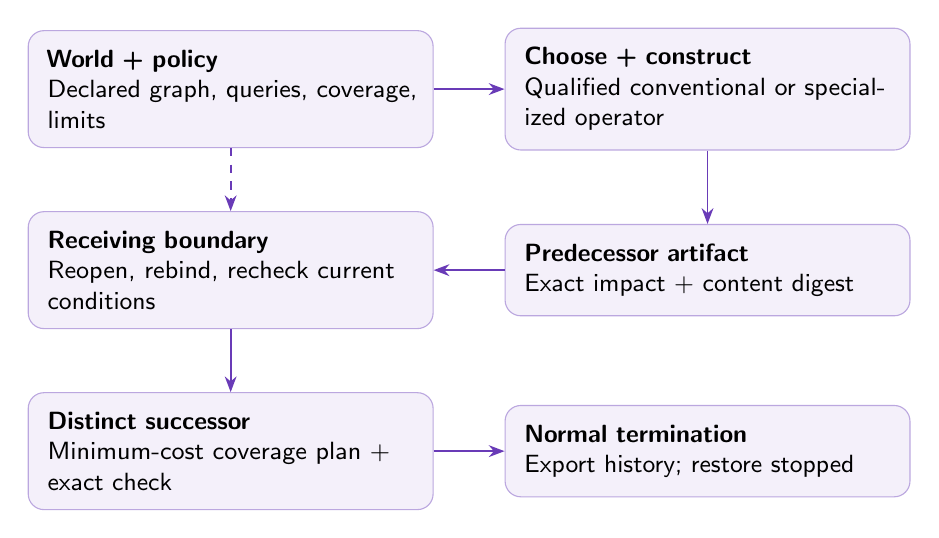
\begin{tikzpicture}[font=\sffamily\small,node distance=8mm and 9mm,
 box/.style={draw=violet!45,fill=pale,rounded corners=2mm,align=left,inner sep=7pt,text width=4.65cm},
 arr/.style={-{Stealth[length=2mm]},draw=violet,line width=.65pt}]
\node[box] (world) {\textbf{World + policy}\\Declared graph, queries, coverage, limits};
\node[box,right=of world] (build) {\textbf{Choose + construct}\\Qualified conventional or specialized operator};
\node[box,below=of world] (check) {\textbf{Receiving boundary}\\Reopen, rebind, recheck current conditions};
\node[box,right=of check] (impact) {\textbf{Predecessor artifact}\\Exact impact + content digest};
\node[box,below=of check] (cover) {\textbf{Distinct successor}\\Minimum-cost coverage plan + exact check};
\node[box,right=of cover] (stop) {\textbf{Normal termination}\\Export history; restore stopped};
\draw[arr] (world)--(build);
\draw[arr] (build)--(impact);
\draw[arr] (impact)--(check);
\draw[arr] (check)--(cover);
\draw[arr] (cover)--(stop);
\draw[arr,dashed] (world)--(check);
\end{tikzpicture}
\caption{The actual dependency is consumed data. Current world, policy, source/environment and authority conditions must hold at the receiver. The dashed edge supplies those current conditions. An intact history does not bypass the receiving boundary.}
\label{fig:architecture}
\end{figure}

\subsection{Seven connected stages, concrete inputs and outputs}
Table~\ref{tab:stages} gives the executed public-demo journey. Native lifecycle family names are exact code values; the correspondence is a local allocation of responsibilities rather than a claim that the names are synonymous APIs. Every stage has a callback, input, returned artifact and explicit check. No transaction is manufactured to make the sequence look complete.

\begin{table}[htbp]
\centering\small
\begin{tabularx}{\textwidth}{@{}p{.97in}p{.95in}YY@{}}
\toprule
Journey & Native family & Concrete work / output & Qualification \\
\midrule
Identify & \texttt{constitution} & Bind objective and supplied case & Finite local scope, authority ceiling \\
Out-Learn & \texttt{evidence} & Read declared dependency structure & Input schema and graph validity \\
Out-Think & \texttt{challenge} & Compare allowed operator work estimates & Same information and palette \\
Out-Design & \texttt{formation} & Construct graph-bound data operator & Payload cap; recorded fallback \\
Out-Strategise & \texttt{admission} & Bind proof, limits and current conditions & Independent exact certificate \\
Out-Execute & \texttt{verification} & Compute impact artifact & Independent answer check \\
Out-Evolve & \texttt{renewal} & Consume impact; produce coverage plan & Exact finite optimum; stop \\
\bottomrule
\end{tabularx}
\caption{Actual public-demo callbacks and native allocations. A future workload with no useful successor should stop after its accepted output; the architecture does not require seven ceremonial operations.}
\label{tab:stages}
\end{table}

The adapter calls the native \texttt{SuccessorStore} operations \texttt{create\_institution} and \texttt{register\_release}. Its \texttt{JobDispatcher} calls are \texttt{seal}, \texttt{dispatch}, \texttt{execute\_tool} and \texttt{complete}~\cite{montrealai2026successorjobs,montrealai2026successorstate}. It also exercises \texttt{SuccessorStore.recover} and \texttt{Journal.verify}, \texttt{backup} and \texttt{restore}. The demonstration has seven completed stages and 48 journal events. Public deterministic fixture signing material is used solely for the local test identities. The declared execution mode is \texttt{synthetic-local}, with \texttt{authority: none}; it supplies no external credential or transaction authority.

The restored record is stopped and globally paused, with zero active proofs and grants. This is a successful restoration of inspectable history, not an automatically runnable successor. The user can inspect and export the record; a new execution still needs applicable artifacts, environment, policy and authorization. An additional schema adapter can produce genuine unsigned project record shapes, but packaging a post-study receipt does not move the earlier scientific preregistration timestamp.

\subsection{Four repositories: verified contribution and remaining gap}
\begin{table}[htbp]
\centering\small
\begin{tabularx}{\textwidth}{@{}p{1.13in}YY@{}}
\toprule
Repository & Verified responsibility and contribution & Actual scope / missing integration \\
\midrule
AGI-Alpha-Agent-v0 & SUCCESSOR records, local dispatcher, journal, backup/restore; foundations and publication surfaces & Native bounded workflow executed. Narrow source snapshot, not full product installation. \\
AGIJobManager & Discovery request interface and Manager USDC accounting route & Source-audited. New graph task not admitted through its installed finite receiver. \\
AGIJobsv0 & Discovery request interface and AGIALPHA jobs route & Source-audited. No external job submission, auction or settlement. \\
AGI-Fleet-Linux & Execution-side boundaries and restore qualification metadata & Source-audited; external execution remains unprovisioned, restore qualification \texttt{NOT\_RUN}. \\
\bottomrule
\end{tabularx}
\caption{Additive use of the actual foundations, without converting interface inspection into a claim of deployed integration. Exact repository commits and source receipts ship with the bundle.}
\label{tab:repos}
\end{table}

Source inspection of Manager, Jobs and Fleet grounds the distinctions in Table~\ref{tab:repos}~\cite{montrealai2026managerreceiver,montrealai2026jobsreceiver,montrealai2026fleetcontroller}. The shared discovery schema is \texttt{successor-discovery-work-request/v1}. Its exact resource fields are \texttt{acquisitions}, \texttt{search}, \texttt{checking}, \texttt{memoryBytes}, \texttt{storageBytes}, \texttt{workerCapacity}, \texttt{installations} and \texttt{elapsedMs}. Binding fields include \texttt{missionId}, \texttt{revision}, \texttt{purposeDigest}, \texttt{charterDigest}, \texttt{modelDigest}, \texttt{sourceDigest} and \texttt{evaluatorDigest}. Manager's route is \texttt{manager-usdc} with six-decimal USDC; Jobs uses \texttt{jobs-agialpha} with eighteen-decimal AGIALPHA. The bounded fixtures declare \texttt{capBaseUnits: "0"} and \texttt{DRAFT\_NOT\_SUBMITTED}. Current installed receivers execute their finite \texttt{inspectCampaign} operation; they do not thereby admit this new graph task. That adapter and qualification work remains missing.

World, policy, proof and authority each answer a different question. \emph{World} binds the declared graph and application order. \emph{Policy} binds coverage eligibility and limits. \emph{Proof} establishes the relevant semantic claim for the current source/environment. \emph{Authority} determines whether the present execution is allowed. A valid answer in an earlier world does not supply any of the other three. Existing held Fleet, Harness and richer-site operations remain held.

\subsection{Five Alpha contracts: source behavior, not performed transactions}
The canonical source names are \texttt{AscensionAccess}, \texttt{NovaSeed}, \mbox{\small\texttt{AscensionRiskOracle}}, \mbox{\small\texttt{AscensionJobMarket}}, and \texttt{AscensionMark}~\cite{montrealai2026ascension}. Their behavior constrains any eventual integration (Table~\ref{tab:contracts}). This edition performs no EVM experiment: the required local toolchain dependencies were absent. The bundle records \texttt{EVM\_NOT\_RUN}. Source inspection is not a contract-test pass.

\begin{table}[htbp]
\centering\small
\begin{tabularx}{\textwidth}{@{}p{1.29in}YY@{}}
\toprule
Contract & Implemented behavior & Boundary for BLOOM \\
\midrule
AscensionAccess & Business, Agent and Validator eligibility combine live ENS and expiring governor admission & A local graph proof grants no contract role. \\
NovaSeed & Transferable ERC-721 genome commits capsule, plan, evidence, parent and job count; no genome/plan setter & A changed immutable Merkle plan needs a fresh seed and explicit authority. \\
AscensionRiskOracle & Stake-backed eligible-validator review, bounded quorum and capacity reservation; green status rechecks eligibility & Risk review is not proof of scientific correctness, demand or profit. \\
AscensionJobMarket & Auction, assignment, submitted evidence, validator voting, payouts and terminal refunds & No auction or settlement is exercised. Missing review quorum can end refunded. \\
AscensionMark & Funded, unexpired, currently green and eligible seed can move from Funding to Bloomed & \texttt{bloom} changes phase, sets execution horizon and emits; it spawns no successor and creates no wealth. \\
\bottomrule
\end{tabularx}
\caption{Verified source responsibilities. The claim is limited to the inspected commits and implementation; no local or external contract execution is reported.}
\label{tab:contracts}
\end{table}

\begin{samepage}
MARK phases are \texttt{None}, \texttt{Funding}, \texttt{Bloomed}, \texttt{Closed}. The job market states are \texttt{None}, \texttt{Auction}, \texttt{Assigned}, \texttt{Submitted}, \texttt{Paid}, \texttt{Failed}, \texttt{Refunded}. Routing checks the committed Merkle leaf and index, budget, current authority and time horizon. A successor that changes the committed plan cannot silently mutate the old seed. Parent lineage is provenance, not permission, proof or finance.
\end{samepage}

Implemented AGIALPHA token behavior covers deposits and payouts, an eighteen-decimal token, a 1\% gross-payout burn and a 5\% validator allocation split between approving validators. These mechanics establish neither a token price nor economic advantage. Manager USDC accounting is a separate route and unit. Proposed incentives or future self-financing mechanisms remain speculative and are not entered as study revenue.

\FloatBarrier
\section{A useful local demonstration}
\label{sec:demo}
The supplied public fixture parses pinned npm lockfiles from Alpha's web client and Manager. It contains 1,136 package-location nodes, 2,000 dependency edges and two application roots. The parser resolves Node-style ancestor locations and local links; an independent acceptance program checks 2,016 declarations/link records. Sixteen unresolved optional peers are disclosed. The larger Jobs lockfile is preserved as source evidence but excluded from this finite demonstration envelope.

Before the demonstration, a reader has static package declarations but no qualified impact index or coverage plan. Afterwards, the reader can choose one of 17 fixed change queries, inspect affected application roots, see the chosen operator and exact qualification, inspect the coverage successor, and export the evidence. For example, a change to \texttt{alpha-web::node\_modules/vite} reaches \texttt{alpha-web::<root>}; the corresponding synthetic plan is \texttt{synthetic-alpha} with weight 7. A Babel-parser path through Babel core and the React plugin gives another inspectable dependency chain. These are declared graph relations, not measurements of tests saved.

The default expert policy chooses conventional reverse indexing for this larger public graph. It qualifies through root ownership, real-edge descending path witnesses and graph-edge closure. All 17 answers match independent acceptance. The complete seven-stage native run takes 1.1277 CPU seconds and 1.1277 wall seconds on the recorded host, including orchestration, checks, journal and restore. This value is deliberately not compared as though it were the same workload as the millisecond synthetic kernels.

\begin{evidencebox}{A short walkthrough}
\textbf{1. Run.} From the extracted study directory, use Python 3.12 with the pinned integration dependencies, then run the public-case command below.\par
\textbf{2. Inspect.} Open the emitted \texttt{index.html}. Choose a changed package. The report shows the affected roots, why the conventional operator qualifies, and the coverage plan that consumes its impact.\par
\textbf{3. Follow the proof.} Read \texttt{summary.json}, the operator, impact and successor artifacts, then the native journal and inactive restoration receipt.\par
\textbf{4. Stop normally.} No deployment, test execution, payment or additional mission is required. The exported record remains available for a later explicitly authorized use.
\end{evidencebox}
\begin{verbatim}
python3 -m pip install -r integration/requirements.txt
python3 demo.py --case public_case/case.json \
  --method expert --output runs/public-demo
\end{verbatim}
The setup step obtains two pinned Python packages and their declared dependencies; the demo itself uses local data and performs no external submission. With prerequisites already installed, the second command is the one-command demonstration. \texttt{python3 demo.py --output runs/bloom-demo} uses the deterministic development fixture instead. An output directory must be fresh so prior evidence is not overwritten.

Users can safely inspect declared dependency impact and finite coverage choices today. They should not use this study alone to suppress real regression tests, approve a deployment, authorize spending or certify a dependency inventory complete. Production use requires representative observed dependencies, measured test coverage and runtime, independently validated correctness, appropriate organization-owned authority, and operational maintenance. None is created by an attractive interface.

\FloatBarrier
\section{Reproducibility, integrity and recovery}
\label{sec:reproduction}
The source-and-protocol freeze was timestamped 2026-10-24 02:02:15 UTC and durably persisted before confirmatory generation and execution. It was then recorded in \href{https://github.com/MontrealAI/AGI-Alpha-Agent-v0/issues/4850\#issuecomment-6378518568}{coordination issue 4850}. The complete SHA-256 identity of \texttt{protocol/FREEZE.json} is
\begin{center}\small\ttfamily
 ecd3df2706d034d17a1441c62fd4dba0c7c9\\
 2f5ea4d22327011bf5e1116bcfbe
\end{center}
The 23 frozen source identities cover the candidate, generator, independent checker, runner, analysis, demo and native integration. Development has two preserved versions and twelve allowed seeds. The first development smoke attempts retain an honest limited console record; complete return values were not retained, a disclosed retention deviation; the later 636 development trial records are complete. No post-confirmation source, analysis, threshold or seed change was used to seek a passing result.

The independently authored checker uses separate BFS and exhaustive subset logic. Its author executes the fresh reproduction before reviewing the original performance statistics, then replays the original deterministic records. All frozen source hashes remain unchanged. The replay excludes timing and host-dependent fields from the equality claim; CPU timing is expected to vary. The reproduction is a different process and authoring role in the same research session, not another institution or concealed benchmark.

The scientific core requires only Python's standard library. The recorded interpreter is CPython 3.12.14. The local native demonstration additionally uses Pydantic 2.14.0 and cryptography 50.0.2. Plotting uses the recorded scientific-Python versions and a fixed generator; every plotted series has a CSV and source digest. The complete archive includes the authoritative PDF, LaTeX, bibliography, vector figure sources, code, protocol, all raw campaigns, analysis, source receipts and an evidence browser. The manifest hashes every included member except itself; the archive digest is recorded externally to avoid a circular self-hash.

\begin{verbatim}
python3 run_study.py --split confirmation \
  --output results/local-confirmation
python3 analyze.py results/local-confirmation
python3 run_study.py --split reproduction \
  --output results/local-reproduction
python3 analyze.py results/local-reproduction
python3 public_case/acceptance.py --check
\end{verbatim}
These commands produce a new reproduction, not additional preregistered evidence for the original claim. Keep the archived receipts and use new named output directories under \texttt{results/}; the cumulative-budget check scans \texttt{development/} and \texttt{results/}. The runner refuses reused output directories. Each rerun adds recorded work without adding new independent worlds. The recorded scientific budget is 1,200 CPU seconds and 256 MiB of new evidence. Bounded local experiments, including failed attempts and all intended exclusions, remain inspectable.

The evidence browser maps major claims to their file, JSON pointer, classification and digest. Its 72 unique scientific worlds are kept distinct from repeated queries, stage counts and replayed executions. The archival checkpoint was reopened and its exact contents verified before confirmation. Final publication assets have independent file digests and a recovery manifest. A standalone document service may change PDF metadata; the exact canonical publication bytes remain inside the verified complete archive. Publication status is established only by the actual repository review and served-asset verification receipt, not by a prospective URL in this paper.

\subsection{Repository and runtime identities}
\begin{table}[htbp]
\centering\small
\begin{tabularx}{\textwidth}{@{}p{1.4in}Y@{}}
\toprule
Source & Pinned Git commit \\
\midrule
AGI-Alpha-Agent-v0 & \texttt{dfc79c4ae81ac612cbff9865a0af8389b6ff3de9} \\
AGIJobsv0 & \texttt{9983478d42c32fe399f28dd9b0e0173f904b8a11} \\
AGIJobManager & \texttt{c5958eae872458c2f3cac48fea0b4bbfadc6ac6c} \\
AGI-Fleet-Linux & \texttt{45759fb096faf8988f58ae5ea71248d0f35a97c7} \\
\bottomrule
\end{tabularx}
\caption{Exact source states inspected and, for the narrow native Alpha snapshot, executed. Later upstream changes do not silently update the scientific artifact.}
\label{tab:identities}
\end{table}

\FloatBarrier
\section{Limitations and the next decisive test}
The finite generator favors small exact graphs and coverage catalogues. Four topologies and shifted sizes exercise controlled variation, not representative software distributions. Authors know the generator and seed ranges. Shared constructors keep access fair but limit conclusions to this implementation, rather than the fastest compiled graph library. The standard candidate and expert choose the same operator, so selector novelty is unproven. The experiment does not test online learned synthesis or unrestricted tool invention.

Proof applies to supplied structure. Deliberately missing edges expose the boundary sharply. Positive synthetic coverage weights are not measured test runtimes, and requirement coverage does not establish fault preservation. The live project demonstration validates parsing, data flow, exact supplied-graph answers and local lifecycle behavior; it is not independent customer validation. The source-only interfaces for Manager, Jobs, Fleet and the contracts have not become an integrated external execution path.

Resource measurement is substantial but incomplete. CPU, wall time, artifact bytes and discrete computational events are recorded; per-method energy, monetary fees, human effort, full resident-memory attribution and maintenance are not. Same-session independent code and execution reduce some implementation risk without replacing external replication. Bootstrap intervals are approximate, and the all-correct sample cannot exclude rare production failures.

The most valuable next study is a preregistered evaluation on unseen public software revisions with observed build dependencies and measured real test coverage and runtime. A conventional regression-selection implementation should remain equally eligible, with human integration time charged. That study would test whether a qualified impact artifact saves an expensive real workflow rather than microseconds of synthetic computation. It should proceed as a new version with new untouched cases and an explicit authority boundary, retaining this edition's failed hypotheses.

\FloatBarrier
\section{Conclusion}
\bloom\ delivers a finite capability that survives export, earns renewed proof, and supplies a distinct coverage-planning successor through actual project runtime components. Exact outcomes, conventional replacement, honest restoration and reproducible evidence are established within the stated envelope. The prespecified competitive advantage, minimum receiver benefit and full-cost commercial viability are not established. The system remains useful because it preserves that distinction in its code, interface, ledger and publication.

Infinite potential is an architectural possibility: a useful accepted artifact may reveal another opportunity. This study executes one justified handoff and then stops. It offers no evidence of infinite growth. \emph{Every successor must earn its proof.}

\section*{Research and artifact statement}
This independent edition builds on the project's published foundations and native infrastructure. Earlier editions and their URLs retain their own identities. Research design, implementation, checking, plotting and manuscript preparation used AI assistance within one coordinated session; distinct checking roles are not claimed to be independent institutions. No external account credentials, security settings, financial commitments or external transactions were changed. Source licenses are preserved, with upstream files and their exact identities listed in the bundle. Operational permission and publication review remain separate from scientific evidence.

\FloatBarrier
\clearpage
{\small\raggedright
\bibliographystyle{unsrtnat}
\bibliography{references}
}
\end{document}
